\chapter{Hybrid Event Recommendation}    \label{ch:recommendation}
\graphicspath{{Part2/Chapter2/figures/}}

Recommendation in online services has gained momentum during the recent past years as a key factor to deliver personalized content. Reducing the information overload and assisting customers to make decision become part of primary concerns in the e-service area. To this aim, recommender systems attempt to provide efficient filters that decode the user interests, and optimize accordingly the information perceived. To help these systems predict items of interest, various clues are available ranging from a user profile, explicit ratings, to past activities and social interactions. For more details, Appendix~\ref{app:recommendation} describes two popular recommendation techniques, namely the content-based recommendation and the collaborative filtering.

Integrating a recommender system in event-based services is a key advantage to attract people attending events and to promote face-to-face social interactions. Indeed, the event recommendation can draw on different features such as the user preferences (ratings, likes, etc.), the attended events (visited places, involved artists), or even the social co-participation. Broadly speaking, the decision making upon attending events depends on some restrictions such as time, location, category, popularity and which friend will attend. However, the existing techniques (e.g. collaborative filtering and content-based methods) cannot cope at all with the complex inherent nature of such decision. In addition, a recommender system is often application-specific, that is, to be tuned according to the item context (e.g. type, reasons to select an item, etc.). Another challenge in our work is that events often involve different topics (e.g. different genres in one musical concert). As a result, the user profile constructed based on the attended events may contain a wide variety of topics. This leads to topically diverse profile that may conceal the effective user interests. 

To tackle these issues, we propose a hybrid recommender system based on Semantic Web technologies~\cite{Khrouf:RecSys2013}. Our belief is that a structured representation presents one solution to cope with the complexity of event-specific characteristics. This modeling will ensure a more straightforward way to explore and reason over the data. It makes possible to ask complex queries, for example, to retrieve events involving the same artist within a specific geographical area. In addition, the semantic model empowers the enrichment of event descriptions with additional information from Linked Data. Such enrichment can provide valuable inputs for the content-based recommender system~\cite{DiNoia:SEMANTICS12}.

In the second step of our approach, we propose to quantify the user interests based on topic modeling technique. The objective is to detect the user propensity towards specific topics. It will be integrated in the recommender system in order to control the impact caused by the diversity of a user profile. Finally, we exploit the collaborative participation assuming that the social information about ``which friend will attend an event'' plays an important role in decision making. In this work, we mainly investigate the extent to which the data enrichment, the social information and the user interests modeling can improve the system performance.


\section{Content-based Recommendation using Linked Data}
\label{sec:linkeddata-recommendation}
The principle of content-based (CB) recommendation is to suggest new items similar to those a user liked in the past. The similarity between items is computed based on the descriptive features of the item using a distance measure such as Cosine similarity, Pearson correlation and Latent Semantic Analysis~\cite{Landauer:1998}. The most common representation of the item is the keyword-based model, in which attributes are represented by weighted vectors of keywords usually computed by TF-IDF scheme (term frequency/inverse frequency). To build such a profile from unstructured data, feature extraction techniques are needed to shift the item description from the original representation to a structured form suitable for next processing (e.g. keyword vectors). This task becomes straightforward by the use of Semantic Web technologies. CB recommender systems can greatly benefit from the ease of ontology-enabled feature extraction, and the availability of Linked Data covering different domains to enrich the item profile. In the following, we explain how to compute the items similarity in Linked Data.

\subsection{Items Similarity in Linked Data}
In order to compute the similarity between items in Linked Data, we resolved to apply the approach proposed by Di Noia et al~\cite{DiNoia:SEMANTICS12}. The key idea is that semantically similar items from RDF graph are the subject of two RDF triples having the same property and the same object (where a triple=$<$subject,property,object$>$). The intuition behind is that: \textit{if two subjects are in the same relation to the same object, this is evidence that they may be similar subjects}. Technically, the approach is based on an adaptation of the classic Vector Space Model (VSM)~\cite{Salton:CACM75}, a well-known technique in Information Retrieval (IR). In this model, similarity between documents and queries is computed using their representative t-dimensional weighted vectors of discriminating terms. The application of VSM in RDF graph projects the Linked Data to 3-dimensional tensor where each slice represents an adjacency matrix corresponding to one property in the ontology. Indeed, the Linked Data network can be defined as a graph $G=(V,E)$ where $V$ is a set of resources and $E$ is the set of properties between resources in $V$. For each property $p$ in the set $E$, the related adjacency matrix presents the linkage between the subjects (on the rows) and the objects (on the columns) from $V$ via $p$. Then, a non null weight is assigned to each entry $X_{i,j,p}$ in the tensor for each existing triple $<i^{th}$ subject, $p^{th}$ property, $i^{th}$ object$>$. Figure~\ref{fig:tensor-slices} shows an example of tensor slices related to some properties, namely: \texttt{lode:atPlace}, \texttt{lode:involvedAgent} and \texttt{dc:subject}.

\begin{figure}
  \centering
  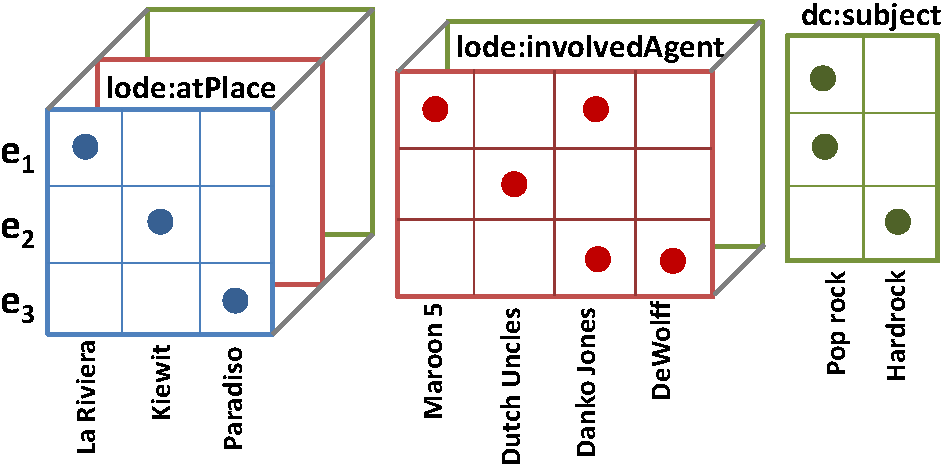
\includegraphics[scale=0.67]{tensor-slices.pdf}
  \caption{Tensor slices of some event properties (place, agent and subject)}
  \label{fig:tensor-slices}
\end{figure}

Assuming that the properties are semantically independent, we would be able to compute the similarity between events according to each property separately. The representation of an event $e_{i}$ according to the property $p$ is a t-dimensional vector indexing the terms/objects related to $e_{i}$ via $p$. The TF-IDF weight of each object $o$ is:

\begin{equation} \label{eq:weight}
w_{o,i,p}=f_{o,i,p} \ \cdot \ log \ \left(\frac {N}{m_{o,p}}\right)
\end{equation}
where $f_{o,i,p} = 1$ if a link exists between the node $e_{i}$ and the object $o$ via the property $p$, otherwise $f_{o,i,p}=0$. $N$ is the total number of events in the dataset, $m_{o,p}$ is the number of events linked to the object $o$ via the property $p$. Then, the similarity between two events $e_{i}$ and $e_{j}$ according to the property $p$ is computed using Cosine distance between their representative vectors as following:

\begin{equation}
sim^{p}(e_{i},e_{j})=\frac {\sum_{r=1}^{t} w_{r,i,p} \cdot w_{r,j,p}} {\sqrt{\sum_{r=1}^{t} w^{2}_{r,i,p}} \cdot \sqrt{\sum_{r=1}^{t} w^{2}_{r,j,p}}}
\end{equation}
This approach can be applied to detect similarity between subjects or objects of RDF triples. It has been successfully used to recommend movies and to improve the quality of content-based system~\cite{DiNoia:SEMANTICS12}. However, it is still limited when the adjacency matrix is very sparse such as the case of matrices associated with \texttt{lode:atPlace} and \texttt{lode:involvedAgent} properties. In fact, such predicates are characterized by the diversity of their object values, thus considered as discriminant properties. For instance, the t-dimensional vector related to \texttt{lode:atPlace} property has only one non-zero weight since an event is typically held at only one venue.


\subsection{Similarity-based Interpolation}

In order to mitigate the sparsity of the adjacency matrix, we propose to interpolate fictitious values based on the similarity between objects. Thus, we initially introduce a discriminability metric (i.e. discriminant power) to gain insight into the properties associated with highly sparse matrices. The metric is defined as following:

\begin{equation}
 Discriminability(p) = \frac{\mid{\{o\mid t=<s,p,o>\ \in G\}}\mid}{\mid{\ t=<s,p,o>\ \in G \mid}}
\end{equation}
where $G$ is the RDF graph, $t$ is the triple representing the link between the subject $s$ and the object $o$ via the property $p$. This formula quantifies the discriminability by the number of different object values on the target property. For instance, from a set of 1700 events (related to 10,323 agents, 627 places and 5,758 subjects), we found a discriminability score of 0.64 for the \texttt{lode:involvedAgent} and 0.45 for the \texttt{lode:atPlace}, while it is only equal to 0.10 for the \texttt{dc:subject} predicate. Furthermore, similar events are not necessary occurred at the same location or featuring the same performers. In order to reduce the discriminability impact, we interpolate fictitious weights in the adjacency matrix based on the similarity between objects as depicted in Figure~\ref{fig:interpolation}. 

\begin{figure}[htb]
  \centering
  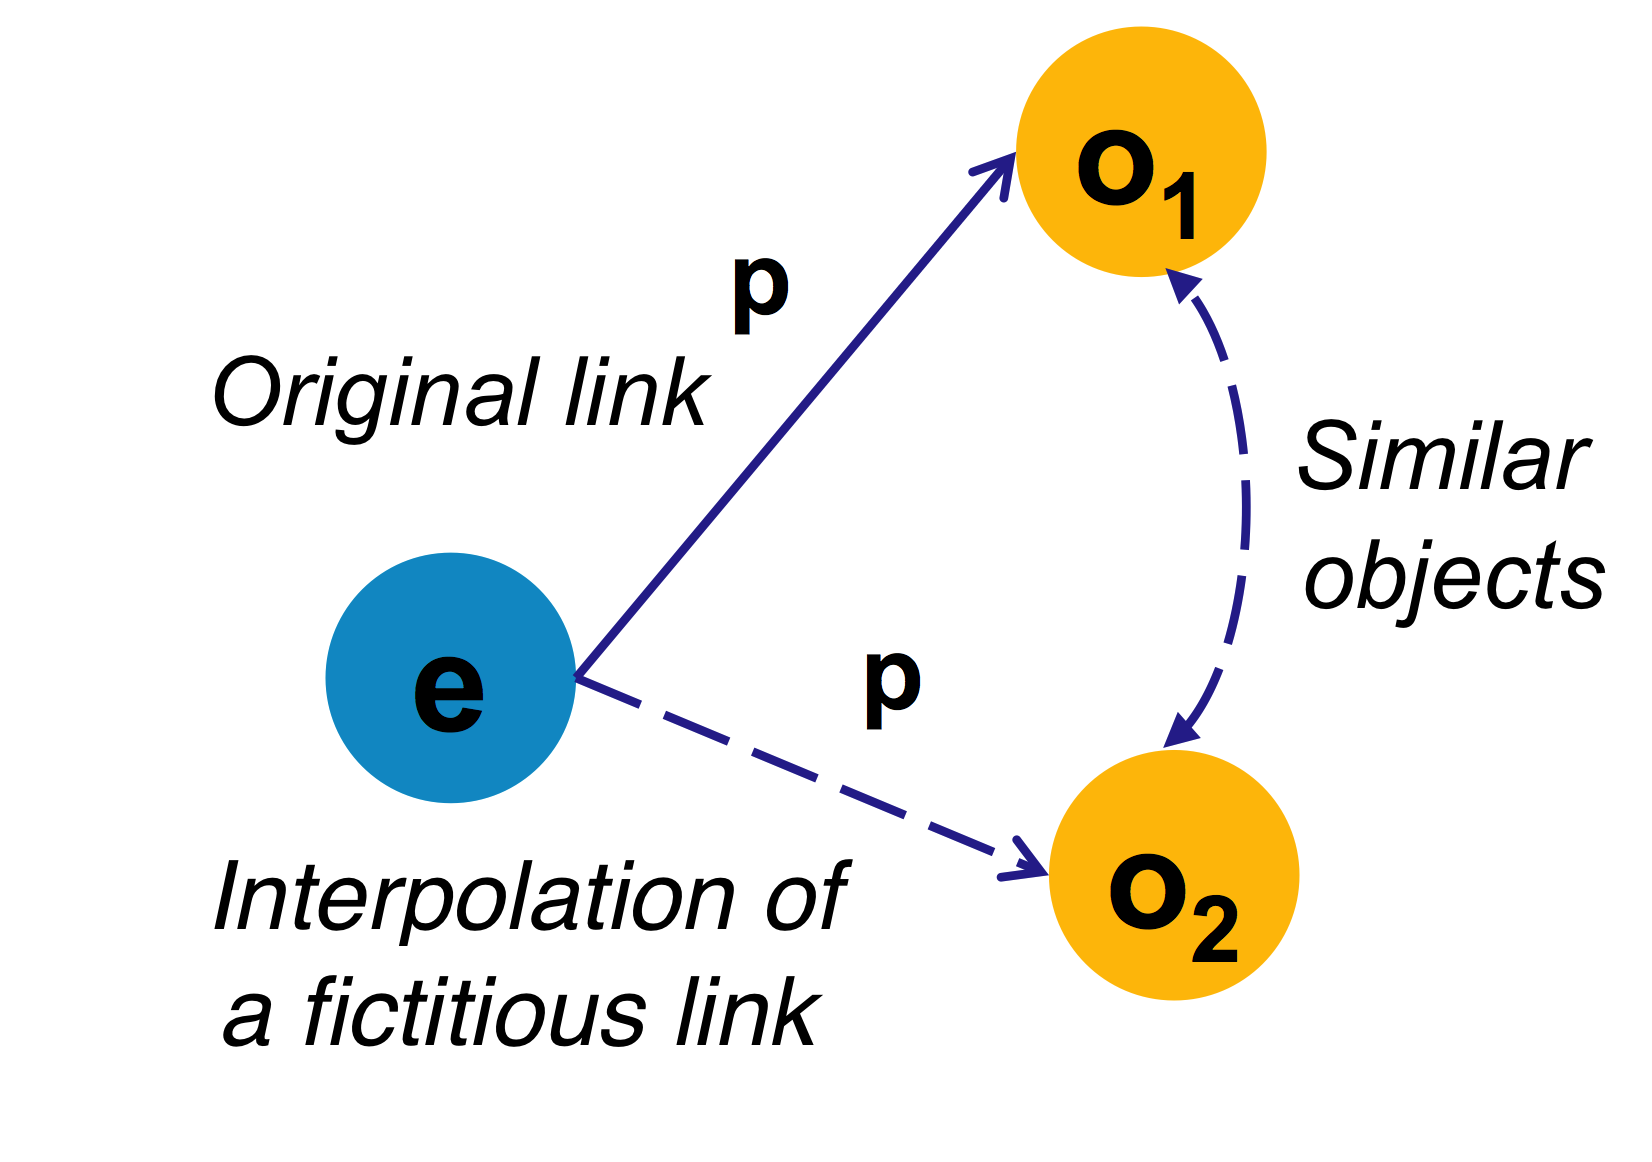
\includegraphics[scale=0.1]{sim-interpolation.png}
  \caption{Similarity-based Interpolation}
  \label{fig:interpolation}
\end{figure}

More precisely, if an object $o_{k}$ is similar to another object $o_{h}$, and if both $f_{o_{h},i,p} = 1$ and $f_{o_{k},i,p} = 0$, then $f_{o_{k},i,p} = sim(o_{k},o_{h})$. Note that $f_{o_{k},i,p}$ reflects the strength of the fictitious link which associates the event $e_{i}$ with the object $o_{k}$ via the property $p$. If the object $o_{k}$ is similar to more than one object originally linked to the event $e_{i}$, the weight $f_{o_{k},i,p}$ will be equal to the highest similarity score. Thus, for each object $o_{k}$, the equation~\ref{eq:weight} becomes:

\begin{equation}
w_{o_{k},i,p}= \max_{o_{h} \in H}sim(o_{k},o_{h}) \ \cdot \ log \ \left(\frac {N}{m_{o_{k},p}}\right)
\end{equation}
where $H$ is the set of objects originally linked to the event $e_{i}$. The intuition behind this formula is that: \textit{if two subjects are in same relations to similar objects, this is evidence that they may be similar subjects}. We do not pay attention to how similarity between objects is computed. In fact, this measure depends on the nature of the object itself and there exist several existing techniques that can be used. In our case, we exploit the similarity scores between agents (i.e. artists) provided by third party services such as Last.fm, and we compute the normalized geographical distance between venues.


%%%%%%%%%%%%%%%%%%%%%%%%%%
%%%  3. Event Recommendation %%%
%%%%%%%%%%%%%%%%%%%%%%%%%%

\section{Event Recommendation }
\label{sec:event-recommendation}
Different from a classic item, events occur at a specific place and during a period of time to become worthless for recommendation. Moreover, while a classic item (e.g. movie, book) continuously receives useful feedback, an event has few rating due to its transiency. In our dataset, these ratings are represented by the binary user-event attendance matrix which has a sparsity rate equal to 98\% (i.e. a set of users attend a very limited number of events). As a solution, one can address event recommendation using CB recommender system that exploits the matching of event attributes with the user profile. This perfectly complies with the constraints considered when it comes to decide whether or not to attend an event. Metadata such as distance, time, topics and artists are important and influential factors in such decision. Still, the CB recommendation might suggest items with a limited diversity and overlook the social information regarding the question ``which friend is going?''. To reduce this gap, we propose to enhance its performance by enriching the content using Linked Data, and by improving the detection of the user interests. Then, we incorporate the social information using Collaborative Filtering (CF) method, thus producing a hybrid recommendation.

%%%%%%%%%%%%%%%%%%%%%%%%%%%%%%%%%%%%%%%%%
%%%  3.1 Content-based Recommendation %%%
%%%%%%%%%%%%%%%%%%%%%%%%%%%%%%%%%%%%%%%%%

\subsection{Content-based Recommendation}
The CB recommender system suggests future events similar to those a user has attended in the past. We assume that there is a sufficient number of past attended events in the user profile to avoid the \textit{cold-start} problem\footnote{The problem to produce good recommendations for new users where nothing is known about their preferences}, which is out of the scope of the present work. In order to predict the participation of the user $u$ to the event $e_{i}$, we combine the similarity values between events as following: 

\begin{equation}\label{eq:rankcb}
rank_{cb}(u,e_{i})= \frac{\sum_{e_{j} \in E_{u}} \sum_{p\in P} \ \alpha_{p}\ sim^p(e_{i},e_{j})}{\mid P \mid\  \cdot \mid E_{u}\mid}
\end{equation}
where $E_{u}$ is the set of past events attended by the user $u$, $P$ is the set of properties shared between two events $e_{i}$ and $e_{j}$, and $\alpha_{p}$ is the weight that reflects the contribution of the property $p$ in the recommendation.

The properties selected to compute the similarity between events are those which are related to the location, subjects (tags) and involved agents (artists). In contrast, the temporal information is not considered in this work and left for future study. Our belief is that temporality could be harnessed to index the recent events in the user profile, thus reducing the computation. Still, there is a need to deeply investigate the impact that the reduction of the user profile has on the system performance. 

\myparagraph{Geographic Closeness}
In recent research study, it has been shown that users generally tend to attend nearby entertainment events~\cite{Quercia:ICDM10}. This fact makes the location a valuable feature in event recommendation. In our approach, we need to measure the similarity between events according to the \texttt{lode:atPlace} property. Thus, we normalize the distance between two locations using a specific threshold $\theta$ which needs to be determined. As the user home is missing in our data, we measure the distance between attended events for each user as depicted in Figure~\ref{fig:attendance-distance}. Note that the attendance rate becomes extremely low from $\theta=80$ Km. We consider that this value is the normalization threshold from which the similarity between events is equal to zero according to the \texttt{lode:atPlace} property.

\begin{figure}[H]
  \centering
  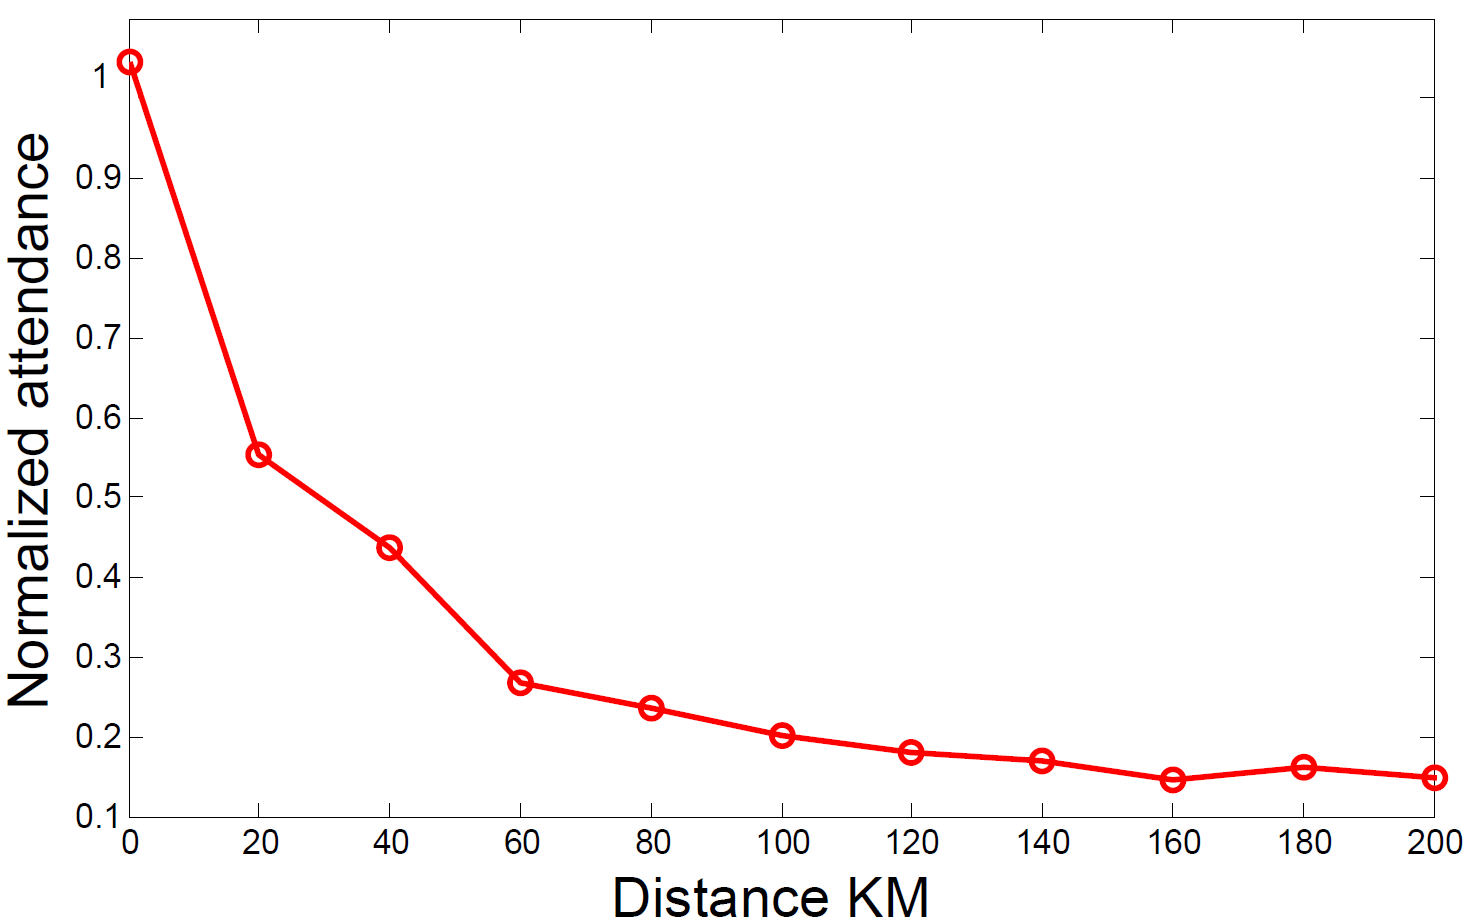
\includegraphics[scale=0.22]{attendance-distance.png}
  \caption{Normalized average attendance per distance}
  \label{fig:attendance-distance}
\end{figure}

\myparagraph{Enrichment with Linked Data} One method to enrich the item profile from Linked Data is to consume background information from DBpedia. The key advantage of DBpedia is the availability of semantically rich data in various domains. Using the mapping between EventMedia and DBpedia, we enrich the topics of an event using the DBpedia topics (e.g. genres) related to the involved artists. More precisely, we retrieve the categories associated with the property \texttt{dcterms:subject} of artists by simply querying the DBpedia SPARQL endpoint\footnote{\url{http://dbpedia.org/sparql}}. The reason behind our interest in DBpedia is that topics are accurately labeled and classified.

\subsection{User Interests Modeling}
One fundamental goal in the recommender system is to suggest new items that best fit the user interests. In our case, this is particularly difficult to achieve due to the presence of topically diverse events. In fact, the real-world social events can be classified into large set of categories ranging from large festivals and conferences to small concerts and social gatherings. When attending an event, the user might be interested in a specific show or artist or might have broad interests. In consequence, relying on event similarity according to the \texttt{dc:subject} property can be influenced by the topical diversity of tags related to events in the user profile. To alleviate this impact, we leverage the Latent Dirichlet Allocation (LDA)~\cite{Blei:MLR03} for detecting the relevant user interests as previously described in Section~\ref{sec:user-interest}.

\begin{figure}[htb]
  \centering
  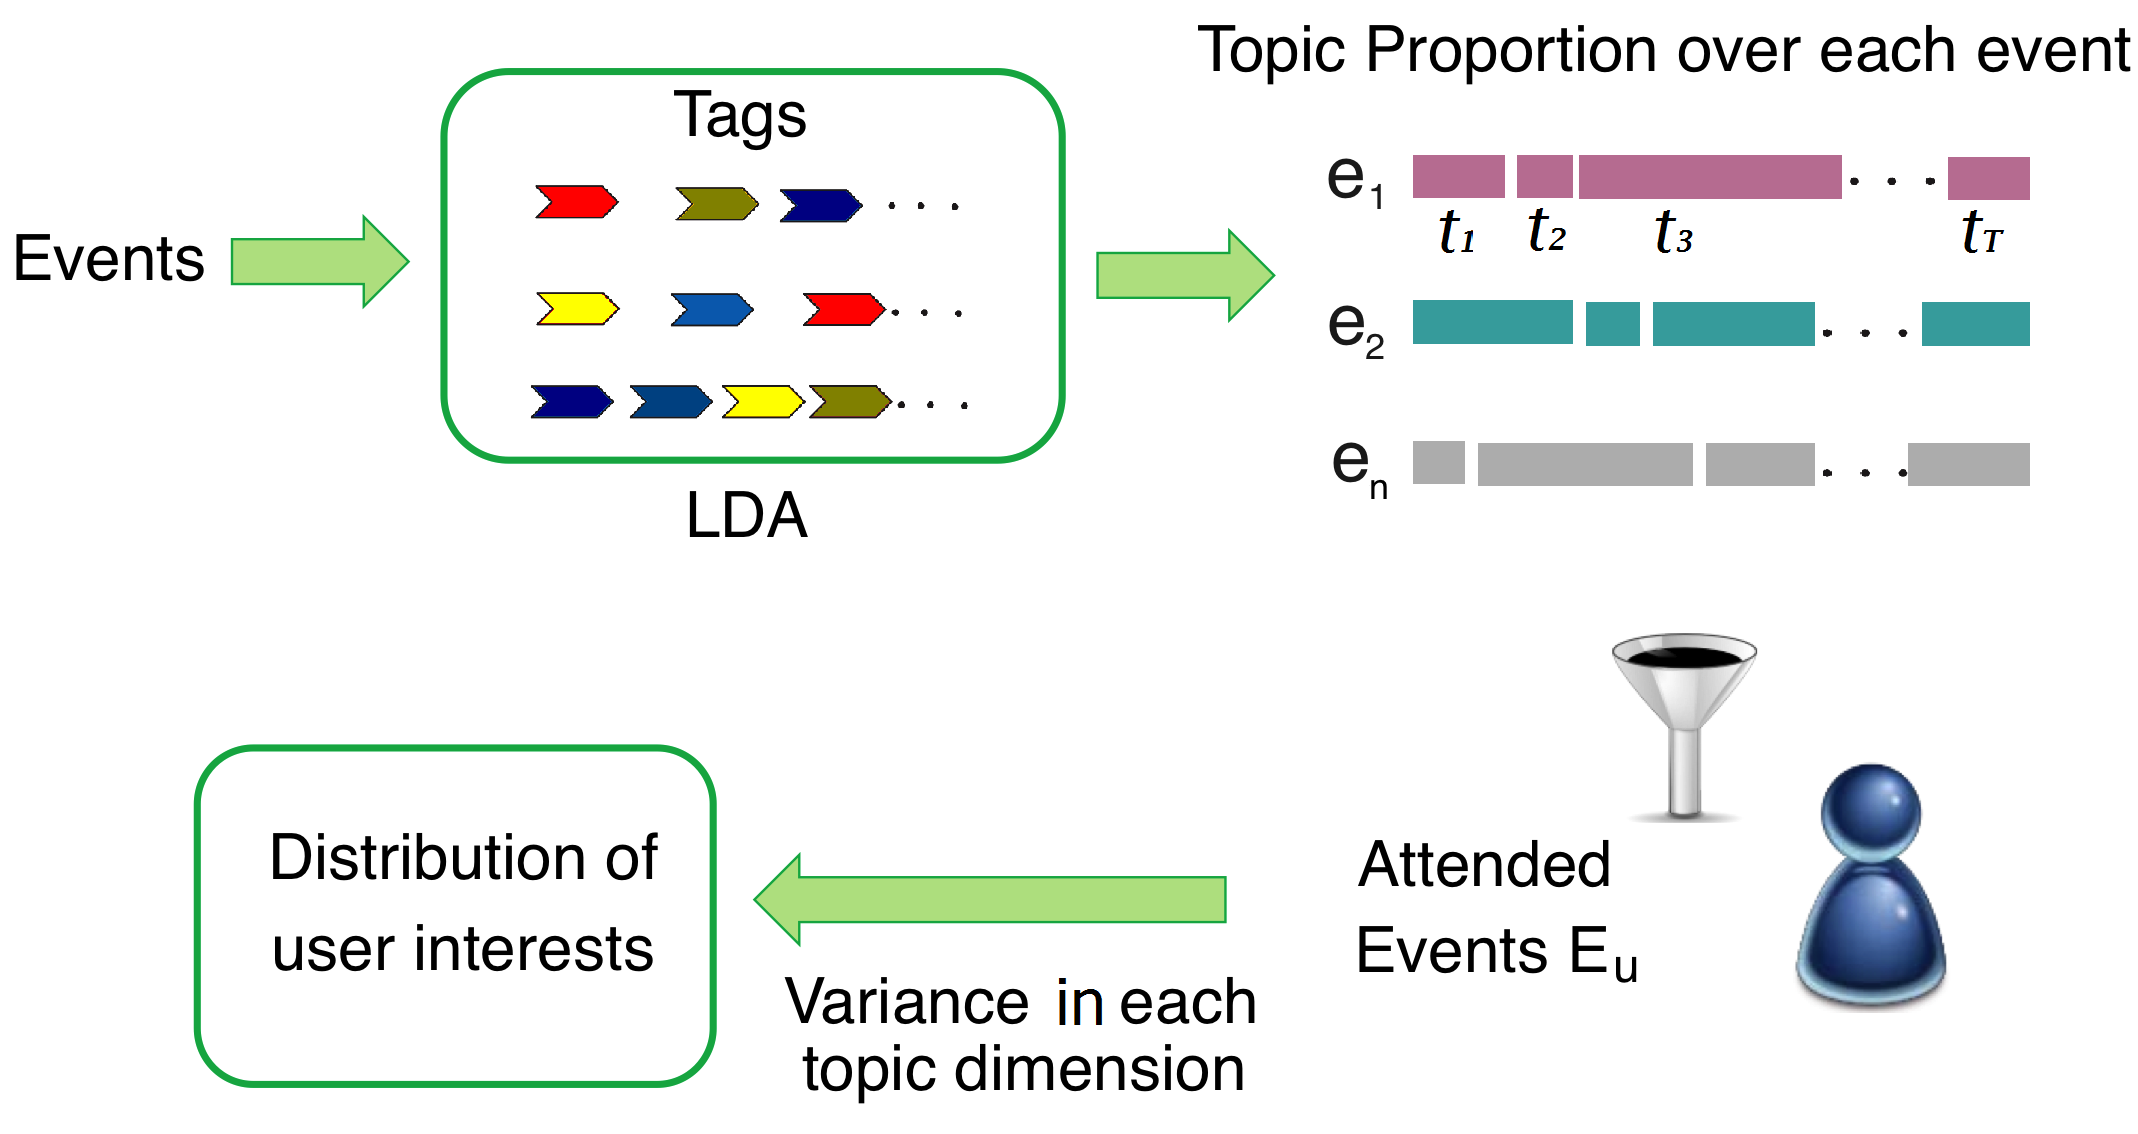
\includegraphics[scale=0.2]{user-div.png}
  \caption{The pipeline of user Interests modeling}
  \label{fig:div-approach}
\end{figure}

Figure~\ref{fig:div-approach} illustrates the pipeline of the user interests modeling. For each event $e_{i}$ having a set of tags, LDA generates a $T$-dimensional vector of topic proportions $\Theta_{i} = [\theta^{1}_{i},\theta^{2}_{i},...\theta^{T}_{i}]$, where $T$ is the number of topics and $\Theta_{i}$ reflects the semantic categories of the event. Then, we compute the variance in each topic dimension $t$ over all the events $E$ attended by a user $\Theta^{t} = [\theta^{t}_{1},\theta^{t}_{2},...\theta^{t}_{E}]$. The diversity score of each corresponding user is the mean of the variances of all the topics dimensions (mean of $\Theta^{1},\Theta^{2}...\Theta^{T})$. 

This approach as introduced by Wu et al.~\cite{Hao:AHJ12} has been originally designed to study the diverseness of individual tastes. But, we think that it is also helpful to detect user's propensity from a topically diverse profile. Indeed, events can be divided into two classes: those related to very few topics or those related to many topics. We consider that events in the first class are those which really exhibit the user interests. Using the variance, we are able to detect high proportions within topic dimension given that this dimension is likely to also contain low proportions (i.e. events are not regularly distributed over the topics).

As an example, Figure~\ref{fig:diversity-scores} shows the normalized diversity scores obtained from a sample of 1,000 Last.fm users. In Figure~\ref{fig:diversity_a}, it is shown that most of diversity scores range from $0.3$ to $0.5$ indicating that users have relatively high interests in specific topics. The diversity scores near to 1 represent users having strong interests in very few topics such as the case of the user plotted in Figure~\ref{fig:diversity_b}. This user has a strong bias specifically towards the topic $9$. Finally, the diversity scores close to zero generally represent the users associated with few attended events (i.e. the cold-start problem).

\begin{figure}[htb]
\centering
\subfigure[]{\label{fig:diversity_a}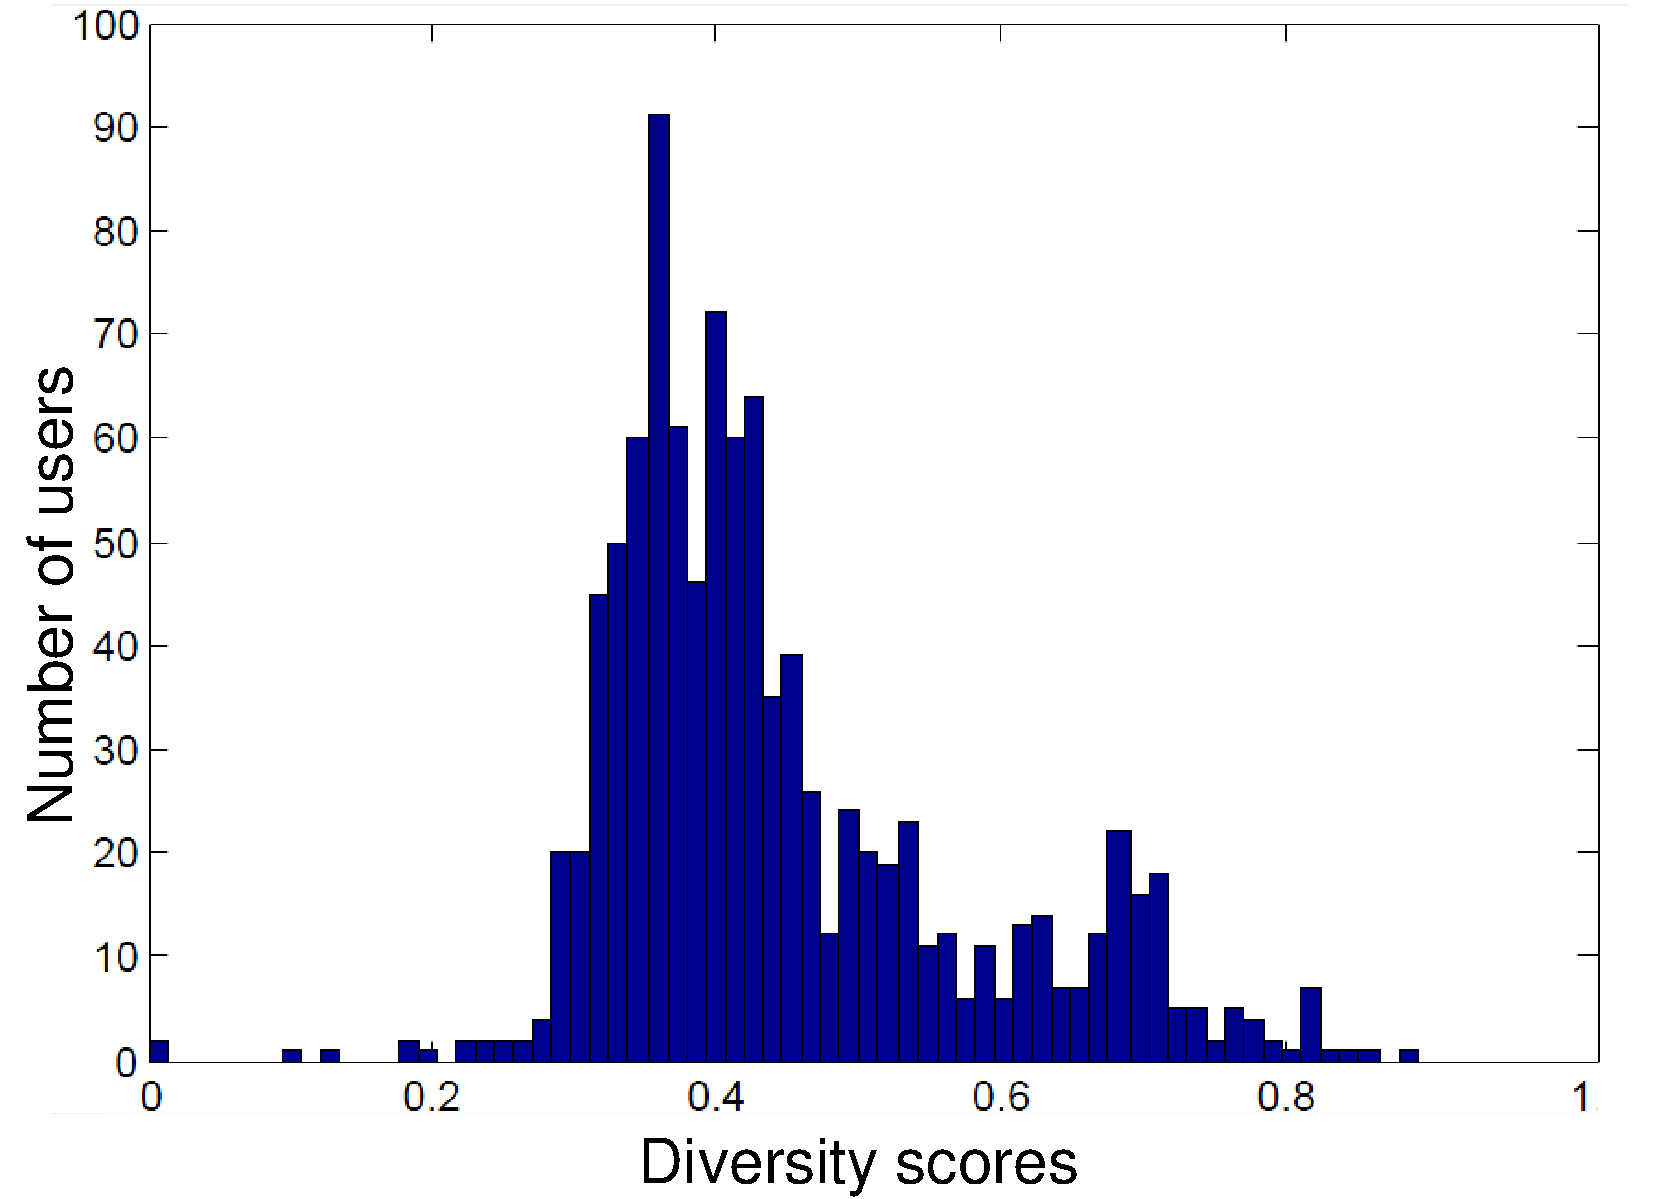
\includegraphics[height=50mm,width=.48\linewidth]{users-diversity.pdf}}
\subfigure[]{\label{fig:diversity_b}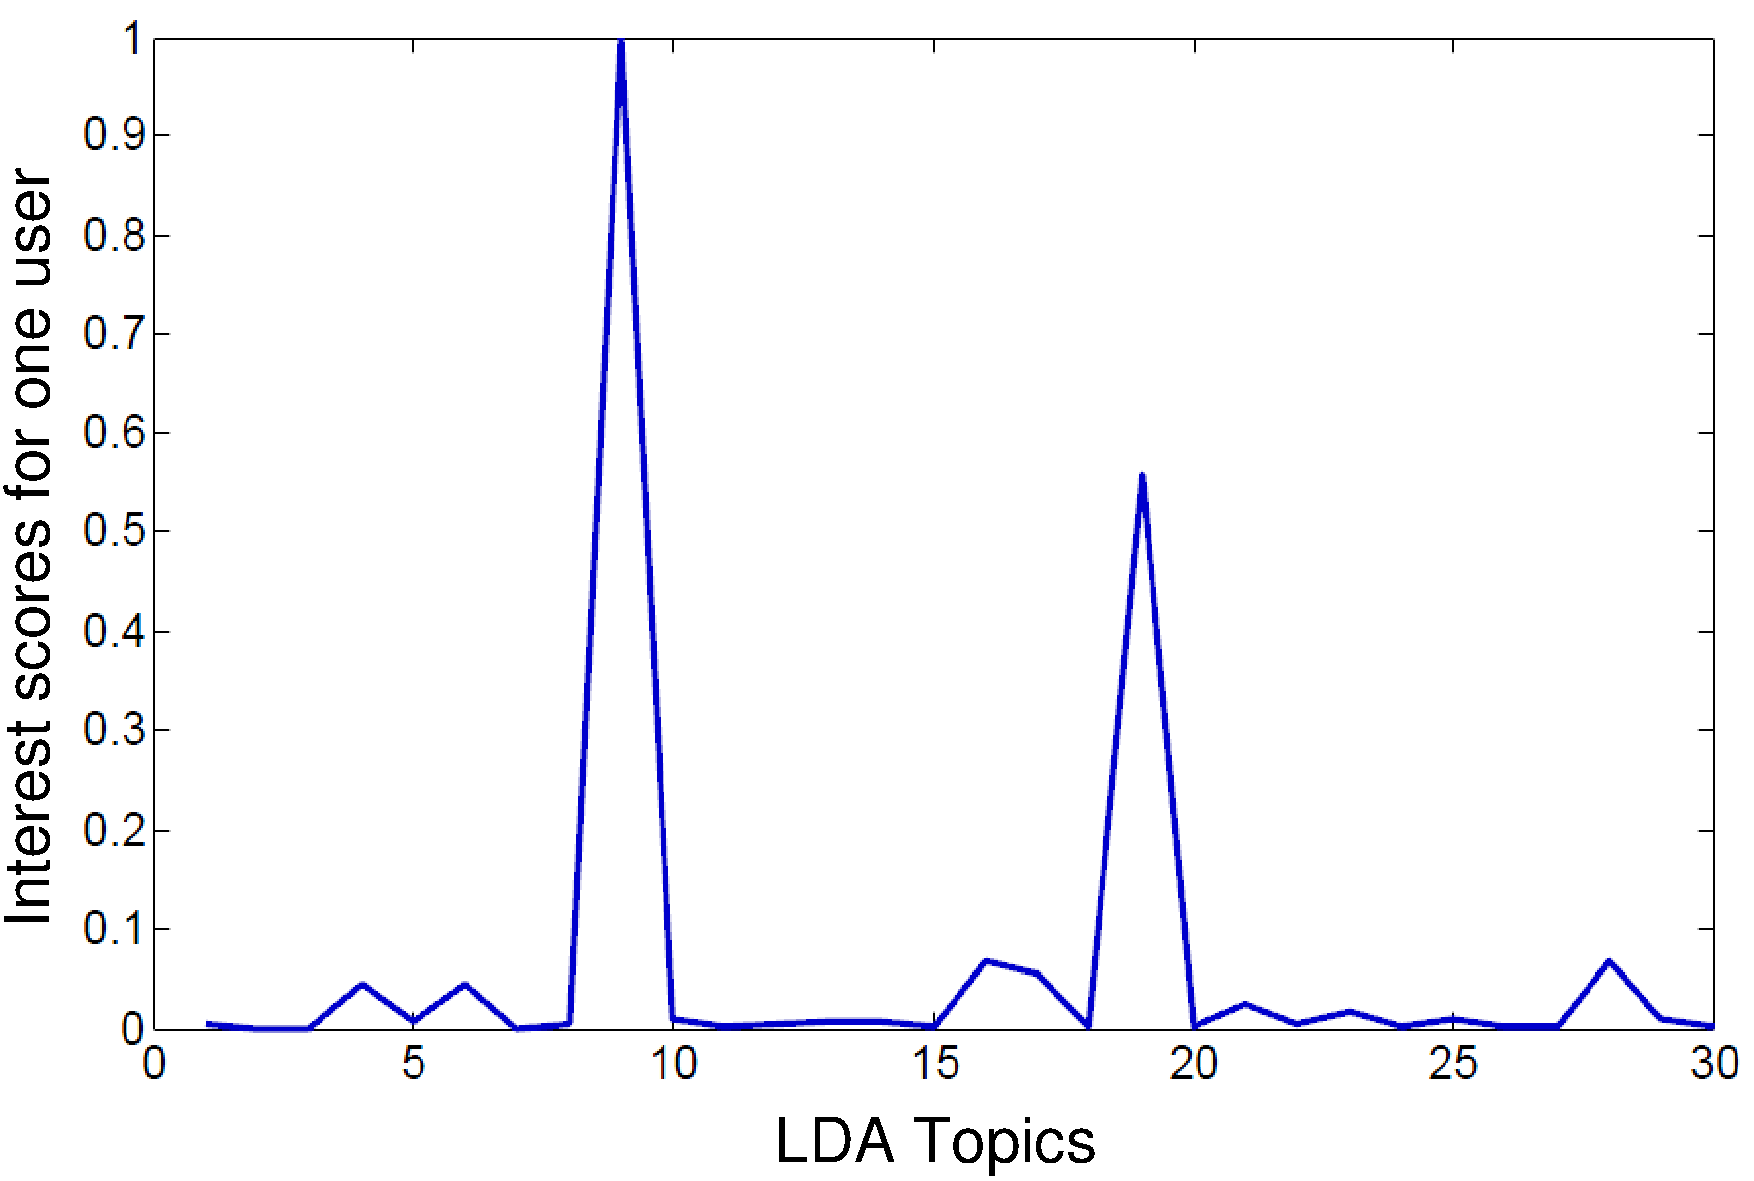
\includegraphics[height=50mm,width=.48\linewidth]{one-user-diversity.pdf}}
\caption{Distribution of topical diversity scores with T = 30: (a) for all the users; (b) for one specific user.}
\label{fig:diversity-scores}
\end{figure}

To take into account the effective user interests in a recommender system, we give emphasis to the events which are more likely to correspond to the user interests. We assign different weights $\beta$ to the events included in the peaks of interest, and to those which are out of these peaks. These weights are then estimated using training methods. The content-based recommendation is extended as following:

\begin{equation}\label{eq:rankcb++}
rank_{cb++}(u,e_{i})= \frac{\sum_{e_{j} \in E_{u}} \sum_{p\in P} \ \alpha_{p}\ \beta_{p} \  sim^p(e_{i},e_{j})}{\mid P \mid\  \cdot \mid E_{u}\mid}
\end{equation}
where $\beta_{p} = 1$ if the property $p$ is different from \texttt{dc:subject}, otherwise the $\beta_{subject}$ is an estimated value depending on whether the event $e_{j}$ corresponds to the user interests or not.


%%%%%%%%%%%%%%%%%%%%%%%%%%%%%%%%%%%%
%%%  3.3 Collaborative filtering %%%
%%%%%%%%%%%%%%%%%%%%%%%%%%%%%%%%%%%%

\subsection{Collaborative Filtering}
A form of social interactions is the collaborative participation such as co-authoring a paper or co-attending an event. In~\cite{Liu:KDD12}, Liu et al. highlight the existence of an offline social network built from the co-attendance of social events. Accordingly, we consider that two users involved in the same event can potentially have a stronger tie than other users. Our assumption is that the more events in which users involve, the stronger is their tie. Thus, the co-attendance can be a clue to provide information at first glance about which ``friends'' will attend an event. Moreover, our dataset contains the users' RSVP that express their intent to join social events, which can be exploited to predict unknown intents. However, unlike the traditional user-based collaborative filtering (CF), we decide to not only consider the similarity between users, but also the contribution of a group of friends. We define the following formula as the prediction that a user $u_{i}$ will attend an event $e$ based on the RSVP of his/her co-attendees (i.e. users who have attended past events with the user $u_{i}$):


\begin{equation}\label{eq:rankcf}
rank_{cf}(u_{i},e)= \frac{\sum_{j \in C } \ a_{i,j}}{\mid C \mid } \ \cdot \  \frac{\mid E_{i} \cap ( \cup_{j \in C } E_{j}) \mid}{\mid E_{i} \mid}
\end{equation}
where $C$ is the set of co-attendees who will attend the event $e$, $E_{i}$ is the set of attended events by the user $u_{i}$, and $a_{i,j}$ is the fraction of common events between the users $u_{i}$ and $u_{j}$ by the cardinality of $E_{j}$. Note that the weight $a_{i,j}$ reflects whether the most of events which are attended by the user $u_{j}$ are also attended by the user $u_{i}$. The rationale behind this formula is two-fold: (1) in the first part, we consider the contribution of each co-attendee individually; (2) in the second part, we consider the co-attendees as a group of friends, and we assume that the more events they attended together with the user $u_{i}$, the more strongly is their relationship.

%%%%%%%%%%%%%%%%%%%%%%%%%%%%%%%%%%
%%%  3.4 Hybrid Recommendation %%%
%%%%%%%%%%%%%%%%%%%%%%%%%%%%%%%%%%

\subsection{Hybrid Recommendation}
To combine the predictions of both CB and CF recommender systems, we propose a weighted hybridization using a linear combination of predicted rank. Taking into account the user diversity and combining the equations (\ref{eq:rankcb++}) and (\ref{eq:rankcf}), we proposed the following function:

\begin{equation}\label{eq:hybrid}
rank(u,e)= rank_{cb++}(u,e) + \ \alpha_{cf}\ rank_{cf}(u,e)
\end{equation}
where $\alpha_{cf}$ is the weight of CF method estimated in conjunction with the weights of CB features using optimization functions for training the system.


%%%%%%%%%%%%%%%%%%%%%%
%%%  5. Evaluation %%%
%%%%%%%%%%%%%%%%%%%%%%

\section{Evaluation}
\label{sec:evaluation}
In this section, we carry out a set of experiments measuring the precision and recall metrics to assess the contribution of each step in our approach, and to evaluate the performance of our system compared with existing approaches.

%%%%%%%%%%%%%%%%%%%%%%%%%%%%%%%
%%%  5.1 Real World Dataset %%%
%%%%%%%%%%%%%%%%%%%%%%%%%%%%%%%

\subsection{Real-world Dataset}
We use the EventMedia dataset and particularly the Last.fm directory which contains a large number of active users. Using SPARQL, we collected 2,436 events, 481 active users whose the attendance rates are within [15,50], generating 12,729 distinct consumption (i.e. user-event pairs). This set of events are related to 14,748 distinct artists, 897 locations and 4265 tags (music domain). For the evaluation, we use a test set containing the most recent 30\% of the consumption and a training test with the remaining 70\% consumption. Then, we measure two metrics used in top-N recommendation task: Precision is the ratio of correctly recommended items and the length of the recommendation $N$; Recall is the ratio of correctly recommended items and the total number of future consumption. Precision and Recall are computed at different $N$ values.

%%%%%%%%%%%%%%%%%%%%%%%%%%%%%%%%%
%%%  4. Learning Rank Weights %%%
%%%%%%%%%%%%%%%%%%%%%%%%%%%%%%%%%

\subsection{Learning Rank Weights}
\label{sec:learning}
To learn the weights of our prediction function, we first test the linear regression with gradient descent that minimizes the least-squares cost function. Then, we use two evolutionary computation methods, namely the Genetic Algorithm (GA) and the Particle Swarm Optimization (PSO) motivated by their success in a wide range of tasks (details in Appendix~\ref{app:optimization}).

%%% Genetic Algorithm %%%

To apply GA in our approach, a chromosome is represented by a vector of the coefficients that need to be estimated. Each chromosome is then evaluated using a fitness function. This function aims to minimize the prediction error and thus maximize the precision of results. Table~\ref{tab:ga-param} shows the GA setting parameters.

\begin{table}[H]
\centering{
\begin{tabular*}{11cm}{c @{\extracolsep{\fill}} ccc}
\hline
Population size & Iterations & crossover & mutation  \\
\hline
30 & 80 & 0.9 & 0.01  \\
\hline
\end{tabular*}
\caption{Setting of GA parameters for event recommendation}
\label{tab:ga-param}
}
\end{table}


%%% Particle Swarm Optimization %%%

As for PSO, a particle is represented by a vector of weights and the fitness function aims at maximizing the precision. Table~\ref{tab:pso-param-2} shows the PSO setting parameters.

\begin{table}[H]
\centering{
\begin{tabular*}{11cm}{c @{\extracolsep{\fill}} cccc}
\hline
Population size & Iterations & $c_{1}$ &  $c_{2}$ & inertia   \\
\hline
30 & 80 & 1.494 & 1.494 & 0.729\\
\hline
\end{tabular*}
\caption{Setting of PSO parameters for event recommendation}
\label{tab:pso-param-2}
}
\end{table}


\subsection{Experiments}
First, we show in Table~\ref{tab:sparsity-tab} the sparsity rates of similarity matrices according to each property. We can see the efficiency of our method to discover latent similarity between events especially for discriminant properties. This highlight the importance of the similarity-based interpolation and the enrichment using Linked Data. Unlike the keyword-based recommender systems, the interpolation is straightforward in our system thanks to the ontology-based data representation.

\begin{table}[H]
\centering{
\begin{tabular*}{8cm}{c @{\extracolsep{\fill}} ccccc}
\hline
Task & location & agent & subject \\
\hline
   (1) & 0.9942 & 0.9174 & 0.3175 \\
\hline
   (2) & 0.6854 & 0.7392 & 0.2843 \\
\hline
\end{tabular*}
\caption{Sparsity rates of the similarity matrices before (1) and after (2) the similarity-based interpolation (for location and agent) and data enrichment with DBpedia (for subject)}
\label{tab:sparsity-tab}
}
\end{table}

Second, we assess the performance of the training methods to learn the coefficients $\alpha$ in the hybrid recommendation algorithm. Note that for this experiment, we do not include the user interests model and we set the $\beta_{subject}$ equal to 1. This experiment aims to rather compare the performance of optimization methods. 

\begin{figure}[htb]
  \centering
  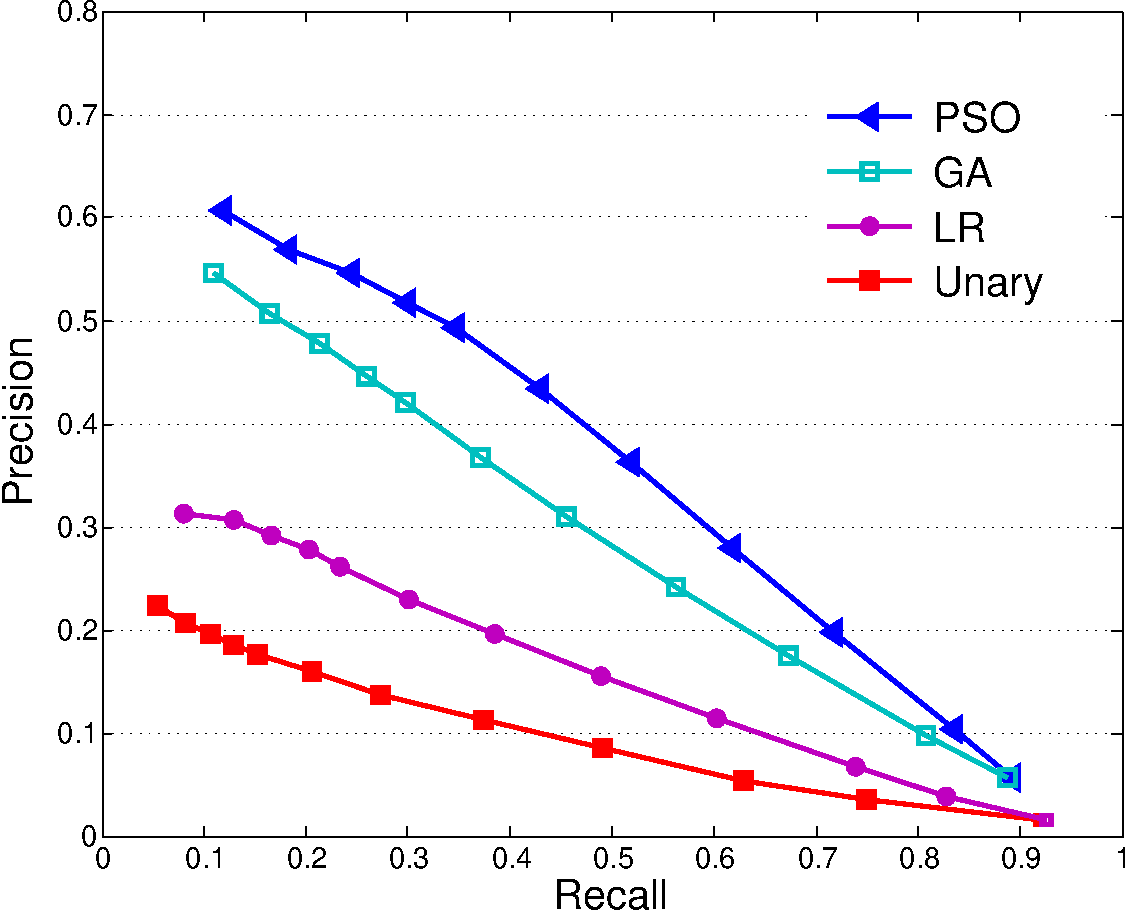
\includegraphics[height=62mm,width=80mm]{training-comparison.pdf}
  \caption{Recall and Precision using different approaches to estimate the vector $\alpha$}
  \label{fig:training-comparison}
\end{figure}

Figure~\ref{fig:training-comparison} shows the Precision and Recall curves. It is obvious that setting all the coefficients equal to 1 achieves the worst performance because there is no adaptive optimization. It is also shown that precision optimization methods (GA and PSO) yield considerably better results compared with error (RMSE) minimization method based in linear regression. This has been also proved in recent work~\cite{Cremonesi:RecSys10} showing that methodologies based on error metrics do not necessarily improve the accuracy of top-N recommendation task. One given explanation is that the RMSE-oriented methods rely only on known ratings to train the system and do not consider the unrated items. Finally, Figure~\ref{fig:training-comparison} highlights the better performance of PSO compared with GA algorithm. We observed a faster convergence to the optimal solution in PSO compared with GA which needs more iterations. This is due to the inherent behavior of PSO where the evolution is only guided by the best particle. In contrast, the GA evolution is guided by a group of solutions in which even weak candidates continue to survive after some iterations. In the following, we use the PSO algorithm to train the system.

To gain insight into the influence of the different steps in our approach, we examine the evolution of the system performance by incorporating in each experiment (by order) the enrichment with DBpedia, the user interests model and the collaborative filtering. Results are illustrated in Figure~\ref{fig:case-comparison}. We can observe that enriching data with DBpedia slightly improves both precision and recall. Indeed, introducing more coherent and qualitative data is one solution to reduce the noise that can be found in the collective knowledge of crowd tagging (e.g. Last.fm tags). Then, the user interests modeling also enhances the system performance. For this experiment, we fix the coefficients $\alpha$ obtained with PSO. Then, we train the system to compute the coefficient $\beta_{subject}$ which depends on the peaks of the user interests. As a result, we obtain $\beta_{subject}$ equal to 0.4 when the event is not included in an interest peak, and $\beta_{subject}$ equal to 1.6 (4 times more) otherwise. This proves the importance to clearly discern the user interests when the user profile contains diverse topics. Finally, combining these results with the collaborative filtering notably increases the recommendation accuracy. Our belief is such improvement is perfectly tangible with the use of a real-world dataset. According to the user centered study presented by Fialho et al.~\cite{Fialho:EVENTS10}, social information such as people and friends who are attending an event has strong priority and influence on decision making.

\begin{figure}[H]
  \centering
  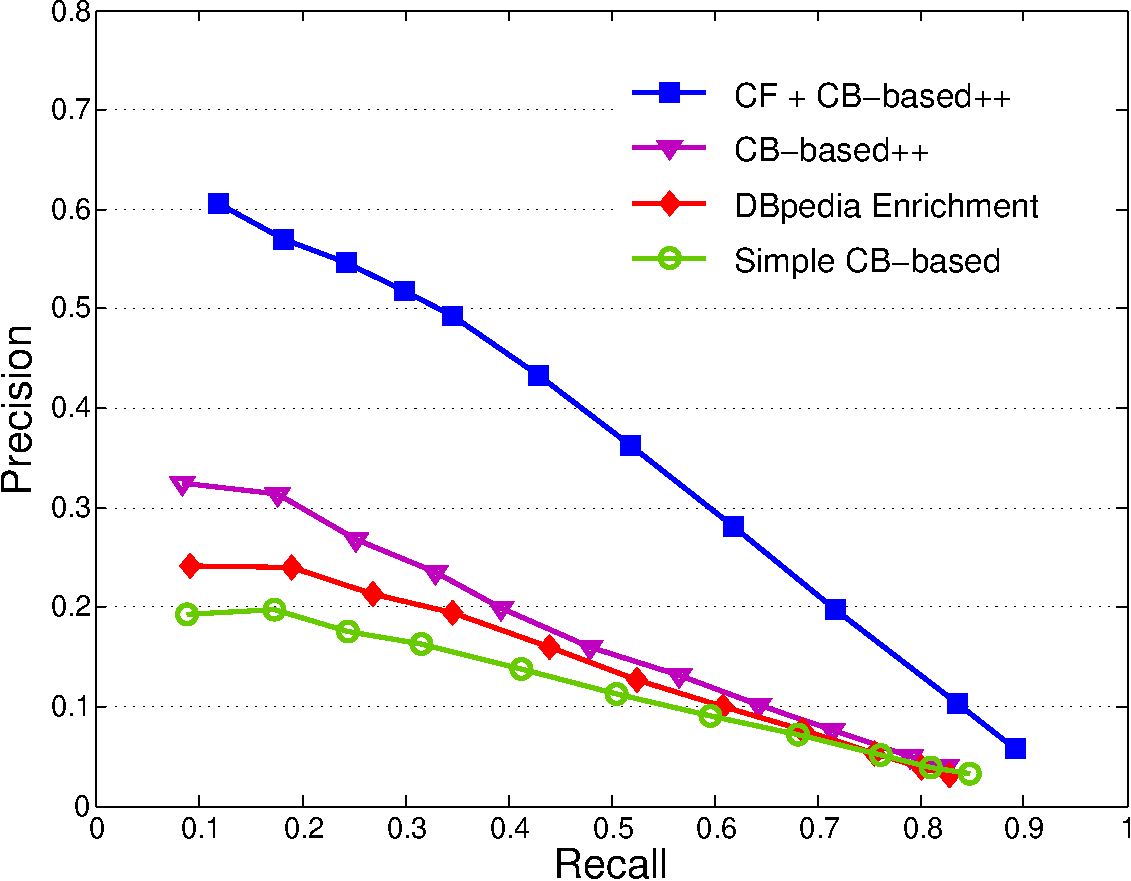
\includegraphics[height=62mm,width=80mm]{case-comparison.pdf}
  \caption{Evolution of the recommendation accuracy by incorporating the DBpedia enrichment, user diversity (CB-based++) and collaborative filtering (CF) }
  \label{fig:case-comparison}
\end{figure}

Lastly, we assess the extent to which a hybrid event recommendation outperforms the existing collaborative filtering based on matrix factorization to detect latent factors from the user-item matrix. We compare our system with the traditional user-based CF and the Probability based Extended Profile Filtering (UBExtended) proposed by Pessemier et al.~\cite{Pessemier:MTA12} to recommend events. This method employs a cascade of two user-based CF systems aiming to recommend the most consumed (i.e. popular) events. The rationale behind is that the probability to consume an event is proportional to the current popularity of the event (i.e. has attracted many users). The comparison results are depicted in Figure~\ref{fig:approaches-comparison}. It is shown that the UBExtended method outperforms the user-based CF algorithm. Still, the hybrid recommendation exhibits the best results in terms of precision and recall. This is due to the benefits of hybridization as has been highlighted in other research studies~\cite{Rojsattarat:2003}.

\begin{figure}[H]
  \centering
  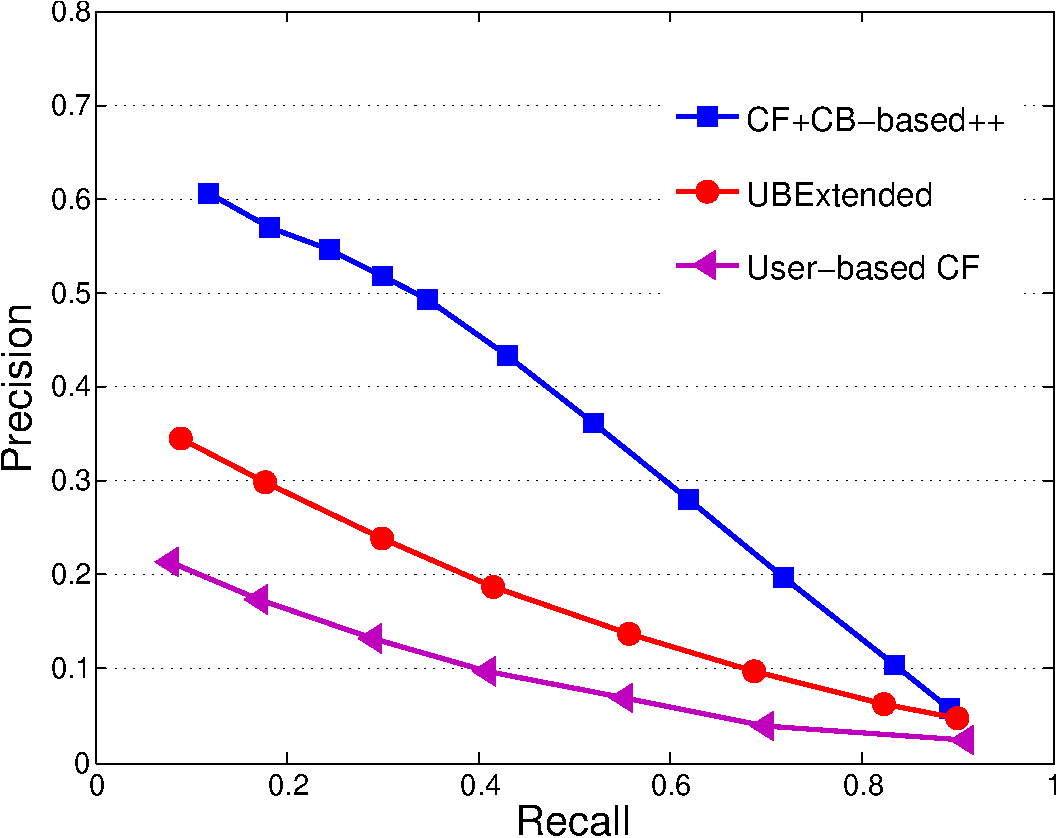
\includegraphics[height=62mm,width=80mm]{approaches-comparison.pdf}
  \caption{Comparison of hybrid event recommendation with pure CF algorithms}
  \label{fig:approaches-comparison}
\end{figure}

\section{Related Work}
\label{sec:related-work}
In the research area of recommender systems, many approaches have been proposed to recommend movies, but few are the studies that deal with event recommendation. Events are particularly hard to recommend due to their short life time and the system often suffers from high sparsity of rating data. Some works have been proposed to overcome these issues and improve the recommendation accuracy. Cornelis et al.~\cite{Cornelis:IICAI05} built a hybrid approach within a fuzzy relational framework that reflects the uncertain information in the domain. The rationale behind is to recommend future events similar to those like-minded users have liked in the past. However, this framework was not evaluated and there is no clear insight about its performance. Minkov et al.~\cite{Minkov:CIKM10} followed the same rationale and proposed a low rank collaborative method to predict the rating of future events. They highlight the performance of the collaborative filtering over the content-based system. Still, their approach was more tailored to recommend scientific talks in the same building and there is no consideration of the geographical constraint. Some other systems have been developed such as ``Pittcult''~\cite{Lee:RecSys08} and ``Eventer''~\cite{Kayaalp:ASONAM09} that position the user within a social network and leverage the trustworthiness between users. Such feature is valuable for recommendation, but it is not available in many systems. Finally, a user centered evaluation~\cite{Dooms:RecSys11} showed that the straightforward combination of CF and CB recommendations outperforms both individual algorithms on almost qualitative metrics such as accuracy, novelty, diversity, satisfaction and trust. Another interesting related works are the recent studies that harness the power of Linked Data in recommender systems. In~\cite{DiNoia:SEMANTICS12}, Di Noia et al. use the Linked Data as the only background knowledge to recommend movies. They highlight the performance of the system that exploits ontology-based data representation compared with the keyword-based representation. Still, there is no deep exploitation of the latent similarity that may exist between movie attributes (e.g. two similar actors).

\section{Conclusion}   \label{sec:conclusion}
In this chapter, we presented an approach for event recommendation combining both CB and CF advantages, and using Linked Data to enrich the event profile. In addition, we proposed an approach to model the user interests and to overcome the topical diversity in the user profile. The evaluation particularly highlights the importance of social information and the user diversity model to enhance the system performance. In the future, we plan to take into account other significant features such as event popularity and temporal indexing of recent consumption.
